\icode[magenta]{E-ME-MU-L4-261018-001}
如图所示，两根长度均为\(L\)的轻质细杆\(a\)、\(b\)将质量为\(2m\)的小球\(P\)和质量为\(m\)的小球\(Q\)连接至固定点\(O\)。细杆\(a\)的一端可绕\(O\)点自由转动，细杆\(b\)可绕小球\(P\)自由转动。初始时\(P\)、\(Q\)与\(O\)点在同一高度。现由静止释放两球,两球在同一竖直面内运动，经过一段时间\(t\)后，细杆\(a\)与竖直方向的夹角为\(\theta\),细杆\(b\)恰好竖直，小球\(Q\)速度大小为\(\sqrt{gL}\)，方向水平向右。已知重力加速度为\(g\),一切摩擦与空气阻力不计。在此过程中，下列说法正确的是\paren[]

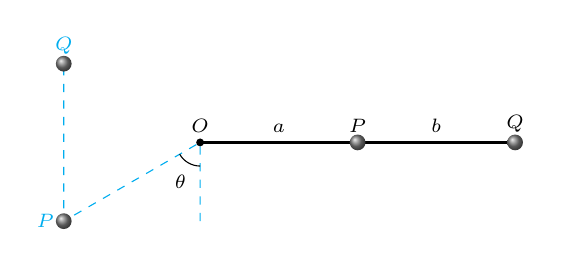
\begin{tikzpicture}[>=stealth,font=\scriptsize]
	\draw[thick] (0,0)node[above]{\(O\)} --node[above]{\(a\)}(2,0)node[above]{\(P\)}--node[above]{\(b\)}(4,0)node[above]{\(Q\)};
	\draw[dashed,cyan] (0,-1)--(0,0)--(-150:2)node[left]{\(P\)}--(150:2)node[above]{\(Q\)};
	\foreach \x in{(2,0),(4,0),(-150:2),(150:2)}
		\shade[ball color=gray] \x circle(.1);
	\fill (0,0) circle(.05);
	\draw (0,-.3) arc(-90:-150:.3);
	\node at(-.25,-.5){\(\theta\)};
\end{tikzpicture}
\begin{choices}
	\item \(\theta =\) \,\qty{60}{\degree}
	\item 当细杆\(b\)竖直时，小球\(P\)的速度大小为\(\frac{\sqrt{gL}}{2} \)
	\item 细杆\(b\)对小球\(P\)做功为\( - mgL\)
	\item 细杆\(b\)对小球\(Q\)的冲量大小为\(m \sqrt{gL} - mgt\)
\end{choices}
\begin{answer}
	AC\qquad 提示：
\end{answer}